\chapter{个人和集体关系}
\par
和前面两章的内容相比这一部分的内容深入到了两国文化的核心内容,有较多的政治历史有关的内容。在我看来文化差异更多的是由历史演变以及经济发展水平形成的。我们打算以个人、集体这两个概念,切入到两国文化差异的核心,比较由于地理环境的因数所导致两国人对个人和集体关系的不同思考,从历史轨迹中比较文化差异的来龙去脉。

\section{现象}

\subsection{职业选择}

专业和职业的选择通常由两个因素影响,一个是自身因素,一个是外界因素。对于自身因素,专业方面和职业上一方面是自身的能力,一方面是个人的兴趣爱好。外界因素上一方面是父母对子女的期望,一方面是社会对人产生的影响。

首先是专业选择,在我们的高中时期,大多数的学生在学习期间并没有也不会考虑对于自己以后大学的专业选择,通常是高考成绩出来,确定了分数,确定了大致的学校,再考虑专业的事情。但是大多数的人并没有什么所谓的对什么专业感兴趣这种概念,没有特定兴趣的,多是与父母交换了一下意见,再在网上或是亲戚处咨询一下选择了就业前景好的热门专业。而有特定兴趣的要是就业前景好也就与上面一样,要是是个冷门专业,可能就会在父母或者亲戚的劝说下改变自己的想法,也有少数人会坚持自己的选择。还有一部分人可能是高考分数到达了目标学校的分数,但是没有到达自己所期望的专业的分数,而又勾选了服从调剂,因此被分到冷门专业。        职业选择与专业选择也是相似。刚到了毕业的时候,大多数的学生,无论是自己还是家人,自然是希望选择待遇好,条件舒适的工作。但是这时和选择专业不同的地方就是能力的大小。专业选择时虽说也有能力的区别,但是总归有大量的与你分数相近的学习与你选择。而选择职业不一样,公司看中你的能力与学历,有能力自然是你挑公司,没有能力,大公司看不上你,小公司又没有前途甚至也可能不要你,很可能就会选择与大学专业无关的工作,可以说是涝的涝死旱的旱死。
\subsection{中国人旅游}

随着旅游业的日渐兴起,无论过不过节,在世界各地,总能看到中国人的旅游大军,分布在世界的各个角落,网上关于中国旅游的话题也是吐槽多多。那么中国人和外国人的旅游到底有什么区别呢?

中国人旅游喜欢扎堆,特别是在节假日出游,到处都是人挤人,尤其在比较有名的旅游景点,你看到的到处都是乌央乌央的人头,毫无放松旅游的感觉。就算是在国外,比如在泰国游玩拍个照的时候,看到的都是一半人和一半景。但是外敷偶人旅游,同样是在泰国,却可能完全不一样,他们大都似电影里演的那样,很休闲的躺在沙滩椅上,晒着日光浴,而旁边还放一杯鸡尾酒。

扎起中国,许多大叔大妈,爷爷奶奶旅游时都强调低价,什么叫做低价。比如说,“999”玩遍泰国,“598港澳游,全程星级酒店”的这类的低价团,都备受追捧。但实际上就算是很正规的旅游团都会存在强迫购物的项目,更不要提这种明眼人一看便知的购物团了。不过在国外旅游,完全没有低价团这件事,往往都需要付足了各种费用,在泰国和越南这种收小费的习惯,其实就是他们养出来的。

中国人旅游爱逛商业街,国内外各地景色不同,但在中国旅游人的眼中,不到商业街就不算是来到了哪里旅游,尤其是以稍老一辈人最为明显,他们不论去哪儿旅游,往往都会在当地的商场里逛一圈,不论是衣服也好,纪念品也好,都很感兴趣。

中国人旅游在国外人看来,都是不可思议的,在国内人看来也是啼笑皆非。不过,这样的旅游方式其实也是非常有意思的。我觉得,作为年轻人,年轻的时候,在选择旅游方式时可以追求点个性。但是等步入了老年,很多人一起热闹旅游也未必不是好事。

近年来,越来越多的中国人都开始讨厌“扎堆”旅游,假日前夕,总有不少人在网上抱怨未来的人流高峰,甚至发誓绝不出门。但实际上,每逢节假日,国内各个主要景点依旧人山人海,人流量永远有增无减,和网上的舆论形成鲜明对比。为什么都抱怨人多,但中国人还是喜欢到人多的地方旅游呢?这是因为从全局考虑,人多也有人多的好处。
\begin{figure}[htb]
    \centering
    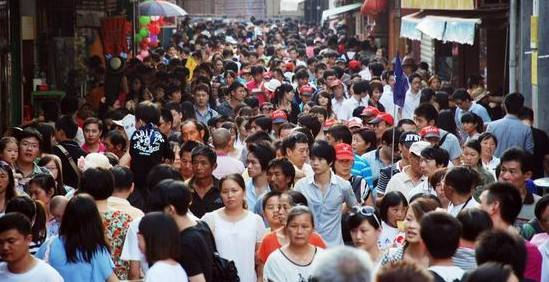
\includegraphics[width=0.6\linewidth]{zgrly}
    \caption{中国人旅游}
\end{figure}





\begin{enumerate}
    
\item \textbf{人多的地方更安全}

许多年轻的旅行者,为了规避人流高峰,喜欢挑选一些人迹罕至的地方去旅游。而人迹罕至,也就意味着这个地方充满了不可知的危险,一旦遇险,你连求援的对象都没有,只能自求多福。而人多的地方,恰恰没有这样的风险。一般来讲,热门景点都已经遭到了完全的开发,排除了大部分未知的危险因素。即便你在这些地方遭到困境,也随时可以向管理人员或身边的游客求助。过去,网上经常有驴友登山失联的消息。试想一下,如果这些山上面到处都是游客,你还会担心失联吗?事实上,在人多的地方,你想要失联都失联不了,因为没走几步,肯定会被人群挤回来。你可能会说,人多难道不是会有踩踏的危险吗?没错,但从统计数据来看,人多地方发生踩踏的概率,远远低于在荒郊野岭被野兽吃掉的概率。再比如说你的手机没电了,在人多的地方就可以很方便的借到充电宝,也是非常幸福的呀。
\begin{figure}[htb]
    \centering
    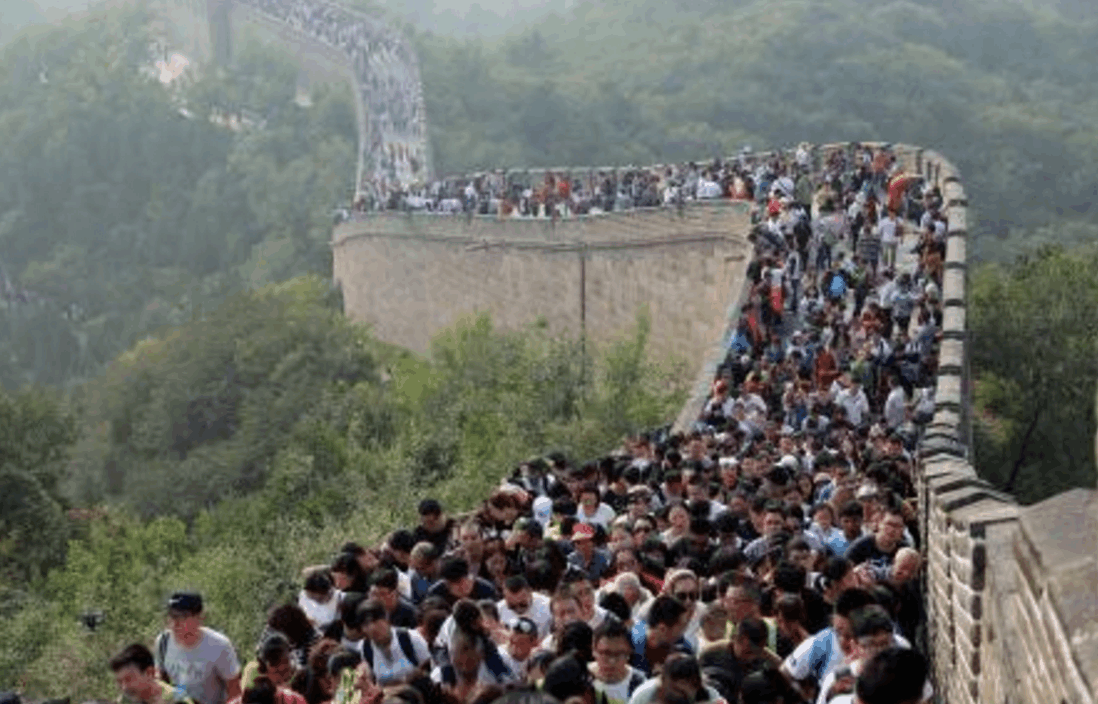
\includegraphics[width=0.6\linewidth]{zgrly2}
    \caption{长城旅游}
\end{figure}





\item \textbf{人多的地方更温暖}

通常情况下,旅游景点的温度,都低于我们平常生活环境的温度。特别是国庆这样的节日,刚好遇到秋季,气温急剧转凉,大家从温暖的室内出来,奔赴山水之间,最大的感受就是真TMD冷。这个时候,如果你去的碰巧是荒无人烟的地方,那么很可能夜里会在帐篷里冻死。 相反,如果你去的是人流密集的场所,几万人身上散发的热量,很快就会把整个地方熏得热火朝天。

\begin{figure}[htb]
    \centering
    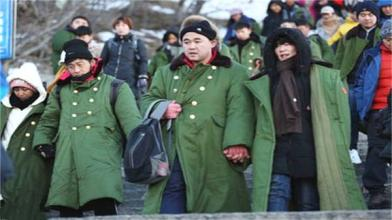
\includegraphics[width=0.6\linewidth]{zgrly3}
    \caption{人多暖和}
\end{figure}



\item \textbf{人多的地方更有趣}

你去那些人群稀少的地方旅游,乍看好像无人打扰,自由自在,但很快你就会陷入空虚和无聊之中。事实上,风景永远是千遍一律的,珠峰上的景色再壮丽,让你在上面独居三十天,是个人都会崩溃。但有一种东西,永远花样翻新,永远不会腻味。没错,那就是人。正所谓“有人的地方就有江湖。”有多少个人,就有多少个江湖。而人多的经典,就好像一个浩瀚的武侠世界。在那些地方,你不仅可以看到美景,而且可以看到身边频频上演的江湖大戏,像情侣吵架、兄弟相争之类的剧目,在景点里随处可见。当然现在最流行的剧目,则是低价旅行团里导游和团客的斗争,揉和了爱情、动作、政治、商战和反乌托邦元素,倍受观众欢迎。去人多的地方旅行,“既是自然之旅,也是人文之旅。”
\begin{figure}[htb]
    \centering
    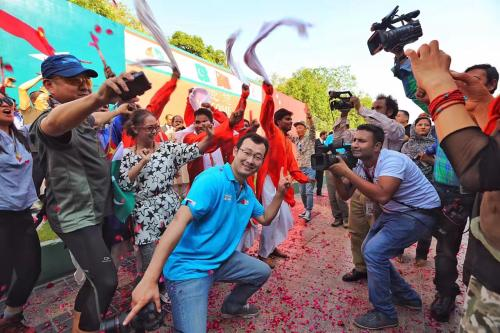
\includegraphics[width=0.6\linewidth]{zgrly4}
    \caption{人多有趣}
\end{figure}


\item \textbf{主要是从众心理作崽}

中国人素来有凑热闹的传统,只是名气大的地方总想也去打卡一番,即使回来不停吐槽也在所不惜。这类游客通常只是喜欢出去玩,但对旅行的认知并没有到很深的层面,除了被其他人走烂的景点,别的地方都没有什么印象。
\end{enumerate}

\subsection{德国人不同于中国人的旅游方式}

生活不止眼前的苟且,还有诗和远方--- 德国人深谙这个道理,在忙碌的工作后安排一场放松身心的旅行对他们来说必不可少。2015年,德国人的度假天数总计高达8.7亿天,由此可知这是一个个酷爱度假的民族。

\begin{figure}
    \centering
    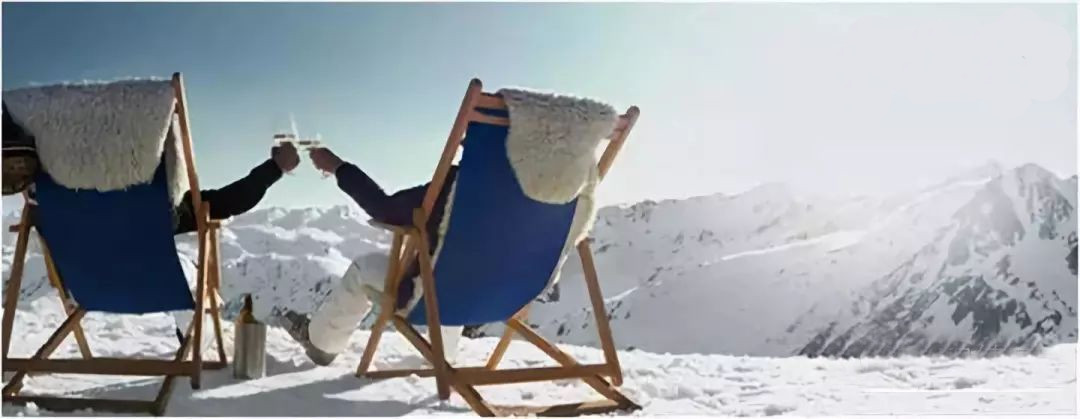
\includegraphics[width=0.6\linewidth]{de_reisen1}
    \caption{德国旅游}
\end{figure}
\paragraph{假日来历:}

“旅游”在全欧或全球范围内都意义重大。对德国人来说,度假可以算最重要的事情之一。人们可以通过度假忘记工作日的疲惫,重新充满能量。“Urlaub(假日)”一词源于中古高地德语“Urloup”。这个词在当时表示上级对某人离开工作岗位的许可。

自1903年起,德国通过带薪休假规定确定了休假天数。那时所有员工都享有三日带薪年休假的权利。早在1841年,德国就出现了由旅游公司Thomas Cook提供的第一个全包旅行。旅客们乘坐火车,从莱斯特到拉夫堡,享受着价格内包含的餐食和乐队演奏等服务。

现在,度假对德国人来说变得更重要了。2013年,全球旅客数量达10.9亿,较2012年增长5\%。旅游行业也得到极大地发展,仅在德国就有300万人从事该行业。



\paragraph{德国假日天数、游客特征:}

现在,德国以年均41天假日和法国在欧洲范围内并列第一,因此德国人和法国人可谓是欧洲的“度假冠军”。就德国而言,除了由雇主保障的30天假日外,在许多联邦州还有额外11天的法定节假日,所以每年德国人常有41天时间供自己随意使用。与之相反,比利时人以年均仅20天带薪假日以及9天法定假日排名垫底。

当德国人出发去度假时,他们当然会做好万全准备。通常来说他们都会带些什么呢?通过什么人们可以一眼就认出德国游客呢?如果德国人准备享受一次火热的夏日风情度假,那么他们首先必备的就是 --- 一顶帽子,帽子可以保护脸部不受阳光暴晒。另外,一个典型德国人在度假时会在脖子上挂一个相机,以便记录下重要的景点风光。穿着方面,他们通常会穿一件衬衫和一条七分裤,必不可少的当然还有一双凉鞋搭配白色袜子。

\paragraph{最受欢迎目的地、住宿方式:}

虽然这有些不可思议,但相比于去别的国家旅游,德国人确实更喜欢留在德国。2015年,像以前一样,德国以29\%这一相当高的比例荣登最受国人喜爱的旅行目的地榜首。2014年,这一比例甚至达到31\%。除此之外德国人也喜欢在欧洲范围内旅行。比如:西班牙以13\%的比例成为最受德国人青睐的国外游目的地,意大利以8.2\%的比例紧随其后。其余较受欢迎的还有奥地利、克罗地亚、希腊和法国等地。

在人们享受应得的假期前,当然得提前订好住宿。那么德国人最喜欢哪种住宿方式呢?对大多数德国人来说,舒服是住宿的第一要义,只有这样他们才能尽可能好地放松,忘记工作日的紧张和压力。另外人们也希望在度假过程中享受到无微不至的服务。所以48\%的德国人选择酒店或舒适的旅馆作为旅行中的过夜地。度假屋以23\%的比例屈居第二。相较起来,帐篷倍受冷落,2015年,只有6\%的德国人选择了此种过夜方式。



\paragraph{度假出行方式:}

在多种不同的出行方式中,开车出行最受德国人青睐,首要原因还在于他们最爱在本国内旅行。因此约有45\%的德国人都喜欢将汽车作为旅行的交通工具。但飞行正行驶在“超车道”上。2015年,约有40\%的德国人乘坐飞机出游。对于前往国外旅游的人,这一比例甚至更高,达到56\%。德国人也会使用公车和铁路交通,不过其占比仅有7\%和5\%。但是现在也有稍稍上升的趋势。相较于国外游,德国人在国内旅游时明显更常使用公车和铁路。



\paragraph{最受喜爱的度假形式\%旅行开销:}

为了能得到尽可能好的休息,德国人特别喜欢在沙滩度假,沙滩之旅以46\%的比例毫无争议拔得头筹。休闲之旅和自然之旅同样也受到他们青睐,分别占比37\%和28\%,差距不大。原则上来说,德国人最爱家庭出游,约有1/4的德国人喜欢和家人一块享受假日。同时探险之旅也很受欢迎,占比24\%,紧随沙滩之旅其后。相反,观光旅行不太受德国人喜爱,仅占比18\%。同样情况的还有徒步旅行,占比17\%。

休假是让人放松的一次奢侈享受,所以德国人用于度假的花费较高。2015年的调查数据显示,如果德国人计划一个5天或更长时间的旅行,平均每人每次旅行的开销为954欧。这一数据较2014年的906欧而言有所升高。平均来看,德国人一次旅行的时间约为12.6天,和2000年相比少了一天。就短期度假旅行而言,德国人一般计划为2到4天,平均每人花销247欧。

\subsubsection{总而言之}

相比于中国人,德国人在旅游有方面更多的追求自由、灵活和探险精神。不同于中国的旅行团的概念,德国人更多的时候以家庭或个人为单位出游。
\subsection{中国的集体主义精神——舍小家,为大家}
\par
新中国成立以来,中国人民为国家建设都有一种舍小家为大家顽强战斗奋力拼搏的精神,留下了许多先进的事迹。最为大家知道的是铁人王进喜,人民公仆焦裕禄等。

\paragraph{铁人王进喜:}
是新中国第一批石油钻探工人,全国著名的劳动模范。他率领钻井队艰苦创业,发扬舍小家顾大家精神,打出来大庆第一块油井,并创造了年进尺10万米的世界钻井记录,为我国石油事业立下汗马功劳。
\paragraph{人民公仆焦裕禄:}
他坚持实事求是、群众路线的领导工作方法,同兰考县全县干部和群众一起,与深重的自然灾害进行顽强斗争,努力改变兰考面貌。他身患肝癌,依旧忍着剧痛,坚持工作,被誉为“党的好干部”、“人民的好公仆”。1964年5月14日,焦裕禄被肝癌夺去了生命,年仅42岁。焦裕禄用自己的实际行动,铸就了亲民爱民、艰苦奋斗、迎难而上、科学求实、无私奉献的焦裕禄精神。
\vspace{1em}
\par
在中国官方的宣传中,上述的这些人物往往作为道德楷模,成为大家学习的榜样。在中国,这样的事迹被认为使人有了一种更高的人生境界,即放弃个人利益,为集体或是全人类的目标而奋斗。因此,集体主义也成为了中国过去几十年激进的社会运动的口号。
%在日常生活中,我们经常可以看见这些宣传标语。这作为一种鼓励我们奋发图强的精神激励着我们努力工作。
\subsection{广场舞}

中国的广场舞起源于中国群众的生活,是一种由人民集体创造的舞蹈形式。它从中国人民群众中来,又到人民群众中去,是一种即具有娱乐意义,同时又兼顾健身锻炼功能的群众自发创造的艺术文化形式。中国广场舞的主要受众是30到50岁之间的中国妇女群众。这些妇女群众就是大家口中著名的中国大妈。中国大妈们十分热爱这项集体运动。她们十数人,或者数十人乃至上百人,集中在空旷的广场上,伴随着具有摇滚和中国特色的流行音乐,跳着步调和节拍一致的舞蹈。而舞蹈的步调与节拍是由大妈们集体商议而来。而种舞蹈的步调与节拍的灵感有的是来自于专业人士的提议,有的则是由大妈们随心随意而作。大家聚集在广场上跳着广场舞,即不需要表现的有多专业,也没有太多规则的束缚。大妈们想来就来,想走就走,想跳就跳。就算大妈们跳错了也不打紧,跳的不好也没人指责。广场舞突出的就是一个集体娱乐性,集体创造性。这种中国式广场舞的文化起点,就是中国集体的农耕文化。中国人习惯了集体活动,在集体中互相帮助,互相学习,共同创造。农耕文化的记忆深深扎根于广大群众的社会生活之中,使得广场舞成为中国人民喜爱的用以宣泄自身情感,展现民族自信,表达民族文化的一种艺术。
\begin{figure}[htb]
    \centering
  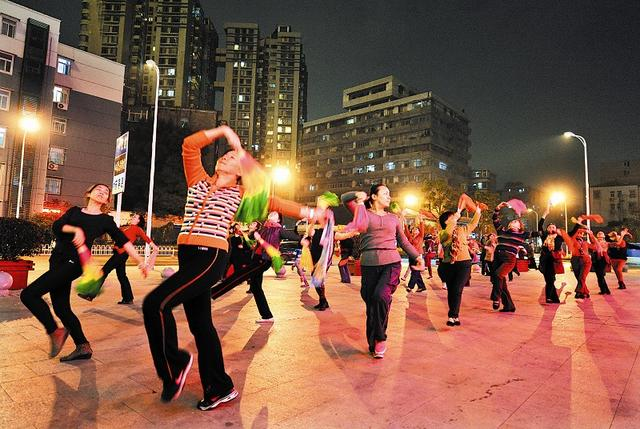
\includegraphics[width=0.6\linewidth]{gcwdm}    
\caption{广场舞大妈}
\end{figure}